\chapter{抽象:进程}
\thispagestyle{empty}

%\section{引言}
在本章中,我们将讨论操作系统所提供的最基本的抽象之一:\textbf{进程}。进程的非正式定义很简单:进程就是一个\textbf{运行程序}[V+65,BH70]。这个程序本身是没有生命的,它只是磁盘中的一堆程序指令(也许还有一些静态数据),等待被执行。而操作系统所做的就是接收这些指令和数据并且让它们运行起来。

事实证明,人们通常希望能同时运行多个程序,举个例子,想象你有一台笔记本或者台式电脑,上面可能同时运行着Web浏览器,邮件客户端,游戏,音乐播放器等等。事实上,一个典型的操作系统(如windows)上可能同时运行着几十个甚至上百个进程。这样可以让操作系统更加易于使用,人们也永远不需要去关心CPU是否可用;
\begin{tcolorbox}[colframe=grey,colback= grey,arc=0pt,left=6pt,right=6pt,top=6pt,bottom=6pt,boxsep=0pt]
\begin{center}
问题的关键\\
如何提供有许多CPU的幻觉
\end{center}
尽管只有几个物理CPU可用,操作系统该如何提供自己有许多CPU的幻觉。
\end{tcolorbox}
操作系统通过\textbf{虚拟化}CPU来制造这种幻觉。运行一个进程,然后停下,接着去运行另外一个,循环往复下去,这样操作系统就可以提供这种有许多CPU的幻觉, 然而实际上只会有一个或者几个物理CPU,这种技术叫做\textbf{时间共享}(CPU时间片技术),这允许用户想运行多少进程就运行多少进程;不过有个潜在的成本就是性能,所以如果CPU必须共享的话,那么每个进程都会运行地相对慢一些。

为了更好地实现CPU的虚拟化, 操作系统需要一些底层的机器指令和一些高级的算法,我们把这叫做机制, 机制包含的底层方法或协议是实现功能的一个必须部分。比如,我们接下来就要学习如何去实现\textbf{上下文切换},
\begin{tcolorbox}[colframe=grey,colback= grey,arc=0pt,left=6pt,right=6pt,top=6pt,bottom=6pt,boxsep=0pt]
  \begin{center}
  时间共享和空间共享\\
  \end{center}
  \textbf{时间共享}是操作系统共享资源的一种基础技术,该技术允许资源被一个实体占用一段时间,然后被另一个实体占用一段时间,循环往复,这些资源(CPU或是网络链路)可以被许多实体所共享。与时间共享对应的是\textbf{空间共享},在空间共享中,资源会被那些想要使用它的实体分割成许多部分,比如,磁盘就是一种空间共享的资源,一旦一个磁盘块被分配给一个文件,那么在用户删除它之前,这个磁盘块通常不会再被分配给其他文件。
  \end{tcolorbox}
即给予操作系统去中断程序运行从而运行另一个程序的能力,这种时间共享机制(分时机制)被所有的现代操作系统所采用。

在这些机制的基础上,操作系统中的还存在一些以策略的形式存在的智能。策略是在操作系统中进行某种决策的算法。例如,给定一些可能在CPU上运行的程序,操作系统应该运行哪个程序?操作系统中的调度策略将作出此决定,可能会依照一些系统历史信息(例如,哪个程序在最后一分钟运行得更多?),负载信息(例如:有什么类型的程序运行了)和性能指标(例如:系统优化交互性能或是吞吐量)做出决定。
\section{抽象:进程}
操作系统对运行程序所提供的抽象是一种叫做\textbf{进程}的东西,就像之前说的,一个进程就是一个的运行程序,在任何时候,我们都可以通过盘点它在执行过程中访问或影响到的系统的不同部分来总结一个进程。

为了理解进程的构成,我们必须了解他的机器状态:程序在运行时可以读写什么。在任何时候,机器的哪些部分对这个程序的执行很重要?

进程的机器状态的一个明显组成部分就是内存。指令位于内存中;正在运行的程序所读写的数据也位于内存中。因此,进程可以寻址的内存(称为\textbf{地址空间})是进程的一部分。

此外,进程的机器状态的一部分是寄存器;许多指令显式地读取或更新寄存器,因此显然它们对进程的执行很重要。

请注意, 有一些特殊的寄存器构成了机器状态的一部分。例如,\textbf{程序计数器}(PC)告诉我们当前在执行程序的哪条指令;类似的,堆栈指针和相关的帧指针用于管理堆栈中的函数参数, 局部变量和返回地址。

\begin{tcolorbox}[colframe=grey,colback= grey,arc=0pt,left=6pt,right=6pt,top=6pt,bottom=6pt,boxsep=0pt]
  \begin{center}
  单独的策略和机制\\
  \end{center}
  在许多操作系统中,一个共同的设计范式是从低级机制中分离高级策略[L+75]。您可以将机制看作是对如何解决系统的问题提供的答案;例如,操作系统如何执行上下文切换?而策略可以看作是为哪个系统问题提供方案;例如,操作系统现在应该运行哪个进程?将两者分开,可以很容易地改变策略,而不必重新考虑机制,因此这是一种\textbf{模块化}形式,这是一种通用的软件设计原则。
  \end{tcolorbox}
最后,程序也经常访问持久存储设备。这样的I/O信息可能包括当前进程打开的文件列表。

\section{进程API}
尽管我们将有关进程实际的API的讨论放到下一章,在这,我们首先给出一些关于操作系统接口所必须了解的一些概念,这些API以某种可用的形式出现在任何现代操作系统中。

\begin{itemize}
  \item \textbf{Create}:操作系统必须包含一些创造进程的方法,当您在shell中输入命令时,或者双击应用图标时,会调用操作系统创建一个新的进程去运行您指定的程序。
  \item \textbf{Destroy}:因为已经有一个创建进程的接口,所以操作系统还需要一个强制销毁进程的接口,当然,许多进程会运行直到它运行结束时自动退出,当它们不自动退出时,用户也许希望直接杀死进程,所以一个用来销毁进程的接口是十分有用的。
  \item \textbf{wait}:有时,用等待的方式让进程停止运行是很有用的,因此,操作系统通常会提供等待的接口。
  \item \textbf{Miscellaneous Control}:除了杀死或是等待(挂起)进程,通常可能还有其他的控制,例如。大部分操作系统提供一些方法去挂起进程(让进程停止运行一会),然后恢复进程(让进程继续运行);
  \item \textbf{Status}:通常有一些接口去获得一些关于进程的状态信息,比如它运行了多久,或是它现在的状态码。
  \end{itemize}
  \begin{figure}[h]
  \centering
  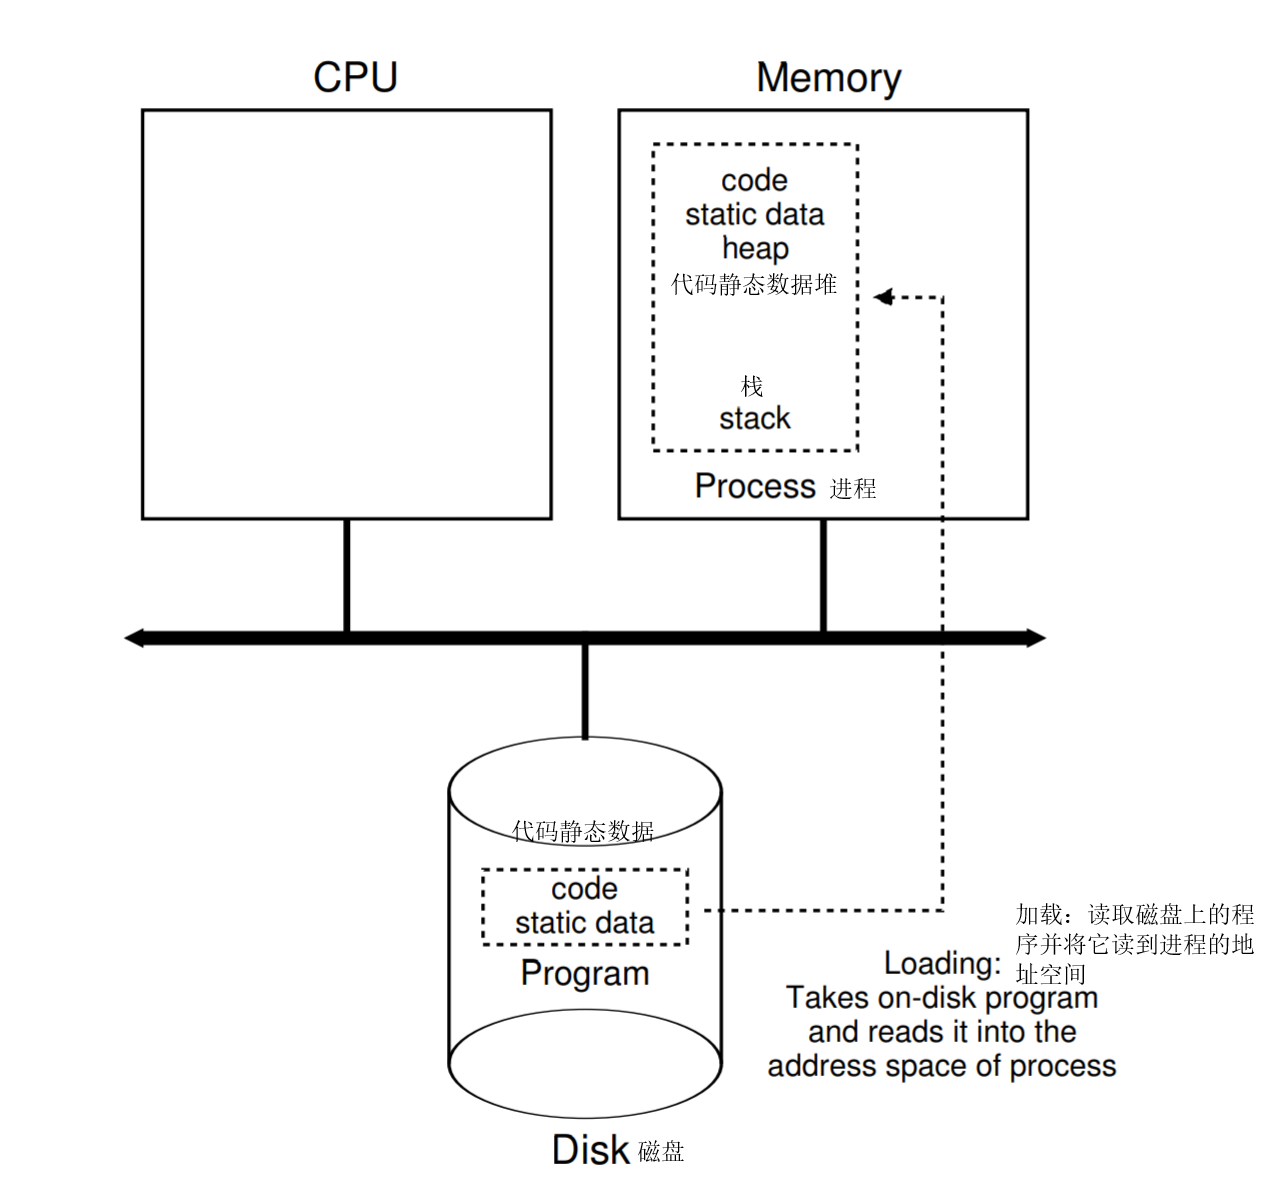
\includegraphics[height=0.5\textwidth]{fig/figure-4-1.png}
  \caption{加载:从程序到进程} \label{fig:figure-4-1}
  \end{figure}   
\section{进程创建:一点小细节}
我们需要揭开的一个谜团是:程序如何转化为进程,具体来说,操作系统是如何启动程序并且运行起来的,进程的创建是如何工作的。

操作系统想要运行程序第一件要做的事情就是将代码和所有的静态数据加载进内存中的进程的地址空间。最初程序是存放在\textbf{磁盘}上(在某些现代系统中,可能是\textbf{SSD})的\textbf{可执行文件},因此,将程序和静态数据加载到内存中的过程要求操作系统从磁盘读取这些字节并将它们放在内存中(如图4.1所示)。

在早期(或简单)的操作系统中, 加载过程是立即完成的,即在程序运行前一次性完成;而现代操作系统是\textbf{延迟加载}的,也就是说在程序执行过程中需要时才会去加载代码或是数据,要真正理解如何延迟加载代码和数据,您必须了解\textbf{分页}和\textbf{交换}机制,这是我们之后讲解内存虚拟化是所讨论的。现在只要记住,在运行任何程序之前,操作系统显然必须做一些工作才能将重要的程序从磁盘转移到内存中。

一旦代码和静态数据加载到内存中,操作系统在进程运行前还会做点小事情。必须为程序的\textbf{运行时堆栈}(或仅仅是堆栈)分配一些内存。您可能已经知道,C程序将堆栈用于局部变量,函数参数和返回地址;操作系统会分配内存并将其中一部分分配给进程,可能还会使用一些参数初始化堆栈;特别的,它会填充main()函数的参数,即argc和argv数组。

操作系统可能还会为程序的\textbf{堆}分配一些内存,在C程序中,堆是用于显式请求的动态分配的数据;程序通过调用malloc()请求这样的空间,并通过调用free()显式地释放它。堆常用于像是链表,哈希表,树或是其他有趣的数据结构,堆最初很小,当程序运行时,通过malloc()库API来请求更多的内存,操作系统可能还会参与其中,并为进程分配更多的内存,以此满足程序的需求。

操作系统还会执行一些其他的初始化任务,特别是有关输入/输出(I/O)的。比如,在UNIX系统中,每个进程默认都会有三个打开的\textbf{文件描述符},用于标准输入,输出和错误;这些描述符使程序可以轻松地从终端读取输入,并将输出打印到屏幕上。我们将在本书中第三部分关于\textbf{持久性}的章节中了解更多关于I/O、文件描述符等方面的内容。

通过将代码和静态数据加载到内存中,创建和初始化堆栈,以及执行与I/O设置相关的其他工作,操作系统已经为程序的执行奠定了基础。它还有最后一个任务;在程序入口点启动程序,即main()。通过跳转到main()例程(通过我们下一章会讨论的专门机制),操作系统将CPU控制权转移给新创建的进程,程序便由此开始执行。

\section{进程状态}
现在我们已经大概了解了什么是进程(我们将继续完善这个概念),以及进程是如何创建的(粗略的),现在让我们来讨论关于进程在不同时间段所处的不同\textbf{状态}。在早期的计算机系统[DV66,V65]中出现了这样一种观点,即进程可以处于这些状态之一。在简化视图中,进程可以处于一下三种状态之一:
\begin{itemize}
\item \textbf{运行态}:在运行态下,进程在处理器上运行。这意味着它正在执行指令。
\item \textbf{就绪态}:在就绪态下,进程已准备好运行,但由于某种原因,操作系统选择在此特定时刻不运行它。
\item \textbf{阻塞态}:在阻塞态下,一个进程执行了某种操作,使它在发生其他事件之前不准备运行。常见示例:进程向磁盘发出了I/O请求,它将被阻塞,因此一些其他进程可以使用处理器。
\end{itemize} 

\begin{figure}[h]
\centering
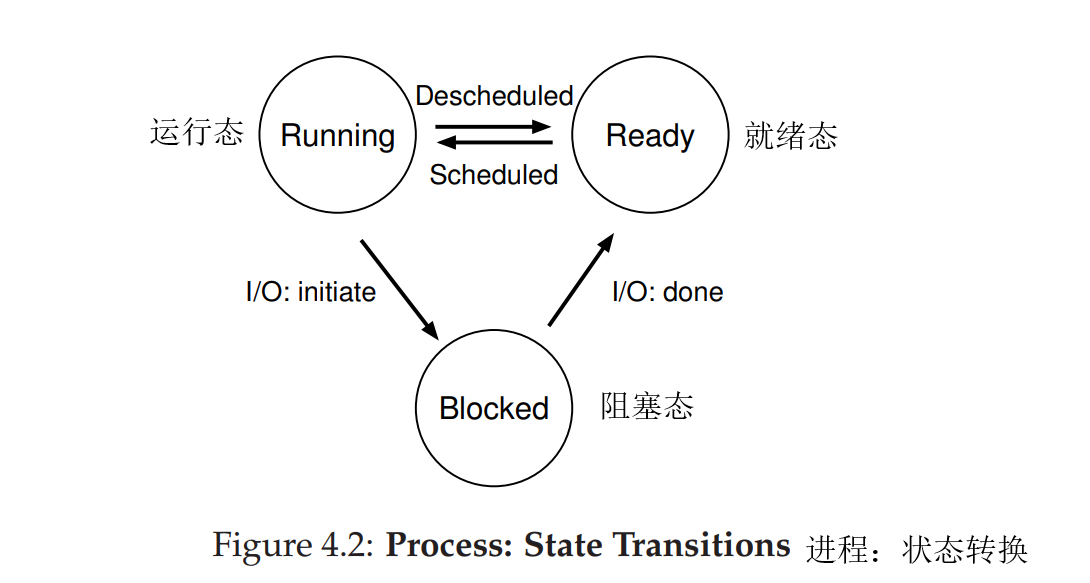
\includegraphics[height=0.5\textwidth]{fig/figure-4-2.png}
\end{figure}   
如果我们将这些状态用图表示,我们将得到图4.2中的图表。正如您在图中所见,进程可以根据操作系统的决定在就绪态和运行态之间切换,从“就绪态”移动到“运行态”意味着进程已经被\textbf{调度执行}从“运行态”移动到“就绪态”因为着进程被\textbf{取消调度}。一旦进程被阻塞(例如,通过启动I/O操作),操作系统将暂停进程,直到某些事情发生(例如I/O操作系完成);此时,进程会再次移动到就绪态(如果操作系统决定继续运行,进程便会立即再次运行)。

让我们看一个例子,来说明两个进程如何通过这些状态进行转换。

首先,假设两个进程正在运行,且每个进程只使用CPU(它们不执行I/O)。在本例中,每个进程的状态跟踪可能如下所示(图4.3)。
\clearpage
\begin{figure}[h]
\centering
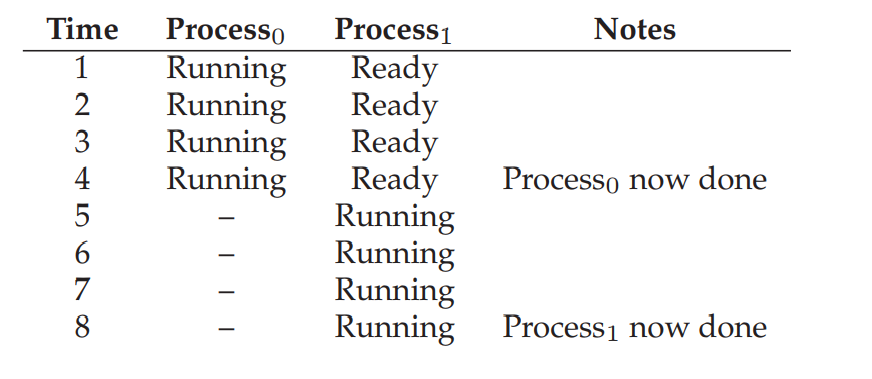
\includegraphics[height=0.3\textwidth]{fig/figure-4-3.png}
\caption{进程状态追踪:CPU} \label{fig:figure-4-3}
\end{figure}
在下个示例中,第一个进程在运行一段时间后发出I/O。此时,进程被阻塞,给另一个进程一个运行的机会。图4.4显示了该场景的跟踪。
\begin{figure}[h]
\centering
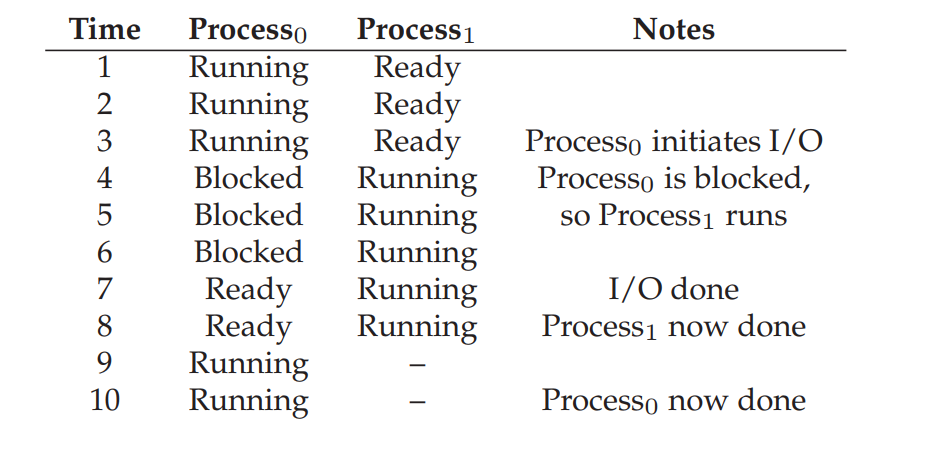
\includegraphics[height=0.3\textwidth]{fig/figure-4-4.png}
\caption{进程状态追踪:CPU和I/O} \label{fig:figure-4-4}
\end{figure}
	
更具体地说,Process 0发出一个I/O请求然后被阻塞,等待I/O完成;进程被阻塞,例如,当从磁盘读取或从网络等待数据包时。操作系统发现Process 0不使用CPU,并开始运行Process 1。当Process 1运行时,I/O完成,将Process 0移回就绪状态。最后,process 1完成,Process 0运行,然后完成。

请注意,即使在这个简单的例子中,操作系统也必须做出许多决定。首先,当进程0发出I/O请求时,系统必须执行进程1,这样做可以保持CPU处于繁忙状态从而提高资源利用率。其次,当I/O完成时,系统会决定不切换回进程0;目前还不清楚这是否是一个好决定。你认为如何?这些类型的决策是由操作系统调度程序做出的,我们将在以后讨论几个章节。

\section{数据结构}
操作系统是一个程序,和任何程序一样,它有一些关键的数据结构来跟踪各种相关的信息。例如,要跟踪每个进程的状态,操作系统可能会为所有已准备就绪的进程放入某种进程列表,并保留一些其他信息来跟踪当前正在运行的进程。操作系统还必须以某种方式跟踪被阻塞的进程;当I/O事件完成时,操作系统应确保唤醒正确的阻塞进程并使其能够再次运行。

图4.5显示了操作系统需要跟踪xv6内核中每个进程的信息类型[CK 08]。类似的数据结构存在于“真实”操作系统中,如Linux、MacOSX或Windows;你可以去查看它们,看看它们有多复杂

从图中,您可以看到操作系统跟踪的有关进程的一些重要信息。对于已停止的进程,寄存器上下文将保存其寄存器的内容。当进程停止时,它的寄存器内存将会被保存到特定的内存位置;通过还原这些寄存器(即将它们的值放回实际的物理寄存器中),OS可以继续运行该进程。我们将在以后的章节中更多地了解这种称为上下文切换的技术。

\begin{lstlisting}
    // the registers xv6 will save and restore
    // to stop and subsequently restart a process
    struct context {
    int eip;
    int esp;
    int ebx;
    int ecx;
    int edx;
    int esi;
    int edi;
    int ebp;
    };
    // the different states a process can be in
    enum proc_state { UNUSED, EMBRYO, SLEEPING,
    RUNNABLE, RUNNING, ZOMBIE };
    // the information xv6 tracks about each process
    // including its register context and state
    struct proc {
    char *mem; // Start of process memory
    uint sz; // Size of process memory
    char *kstack; // Bottom of kernel stack
    // for this process
    enum proc_state state; // Process state
    int pid; // Process ID
    struct proc *parent; // Parent process
    void *chan; // If non-zero, sleeping on chan
    int killed; // If non-zero, have been killed
    struct file *ofile[NOFILE]; // Open files
    struct inode *cwd; // Current directory
    struct context context; // Switch here to run process
    struct trapframe *tf; // Trap frame for the
    // current interrupt
    };
\end{lstlisting}
                图 4.5:xv6 数据结构

从图中还可以看到,除了运行态、就绪态和阻塞态之外,进程还可以处于其他一些状态。有时候,系统会有一个初始状态,当它被创建时,进程就在这个状态中。此外,进程可能处于退出但尚未清理的最后状态(在基于UNIX的系统中,这称为僵尸状态1)。这种最终状态非常有用,因为它允许其他进程(通常是创建进程的父进程)检查进程的返回代码,并查看刚刚完成的进程是否成功执行(通常,程序在基于UNIX的系统中成功完成任务时返回零,否则返回非零)。完成后,父进程将进行最后一次调用(例如,等待(),等待子进程的完成,并向操作系统指示它可以清理任何引用到已灭绝进程的相关数据结构。

\begin{tcolorbox}[colframe=grey,colback= grey,arc=0pt,left=6pt,right=6pt,top=6pt,bottom=6pt,boxsep=0pt]
\begin{center}
旁白:数据结构-进程列表\\
\end{center}
操作系统中充斥着各种重要的\textbf{数据结构},我们将在旁白中讨论这些结构。\textbf{进程列表}(也称为任务列表)是第一个这样的数据结构。这是一个简单的结构,但是任何能够同时运行多个程序的操作系统都会有类似于这个结构的东西,以便跟踪系统中所有正在运行的程序。有时,人们将存储进程信息的单个结构称为\textbf{进程控制块}(ProcessControlBlock,\textbf{PCB}),这是一种包含每个进程信息的C结构的奇特方法(有时也称为\textbf{进程描述符})。
\end{tcolorbox}

\begin{tcolorbox}[colframe=grey,colback= grey,arc=0pt,left=6pt,right=6pt,top=6pt,bottom=6pt,boxsep=0pt]
\begin{center}
旁白:关键进程管理\\
\end{center}
\begin{itemize}
\item \textbf{进程}是正在运行的程序的主要操作系统抽象。在任何时候,进程都可以用状态来描述:\textbf{地址空间}中的内容、CPU寄存器(包括\textbf{程序计数器}和\textbf{堆栈指针}等)的内容,以及关于I/O的信息(例如可以读取或写入的打开的文件)。
\item \textbf{进程API}可由与进程相关的调用组成。通常,这包括创建、销毁和其他有用的API。
\item 进程存在许多不同的状态,包括运行、就绪和阻塞。不同的事件(例如,调度或去调度,或等待I/O完成)会将进程从这些状态中的一种转换到另一种状态。
\item \textbf{进程列表}包含了系统中所有进程的信息。每个条目都存放在\textbf{过程控制块(PCB)}中,PCB实际上只是一个包含特定进程信息的结构体。
\end{itemize}
\end{tcolorbox}

\section{总结}
我们介绍了操作系统最基本的抽象:进程。它很简单地被看作是一个正在运行的程序。考虑到这一观点,我们现在将继续深入讨论细节:实现进程所需的低级别机制,以及高级策略来智能化地控制进程。通过将机制和策略结合起来,我们将建立对操作系统如何虚拟化CPU的独特理解。

